\section{Experiments and Evaluation}
\label{sec:exp}
\begin{table}%
\centering
\begin{tabular}{|l|c|c|}
\hline
Model & Train Accuracy & Test Accuracy \\
\hline
Logistic Regression & $0.9578$ & $0.9461$ \\
\hline
Bernoulli NB & $0.7285$ & $0.7212$ \\
\hline
Ridge Classifier & $0.9419$ & $0.9064$ \\
\hline
Linear SVC & $0.9712$ & $0.9527$ \\
\hline
\end{tabular}
\caption{Sentiment classification accuracy of YouTube comments}
\label{tab:accuracy}
\end{table}

In this section, we present our experimental methodology, evaluation metrics and the results of the experiments. In all of the experiments, we used cross validation to pick the model with the best performance. Namely, we discuss how the data was split into train, dev and test sets, but the results are reported only on train and test sets.

\subsection{Sentiment Analysis}
\label{sec:sent-exp}
\begin{figure*}[thb]%
\centering
\begin{tabular}{cc}
\subfloat[Precision vs. Recall for Logistic Regression \label{fig:pr-lr}]{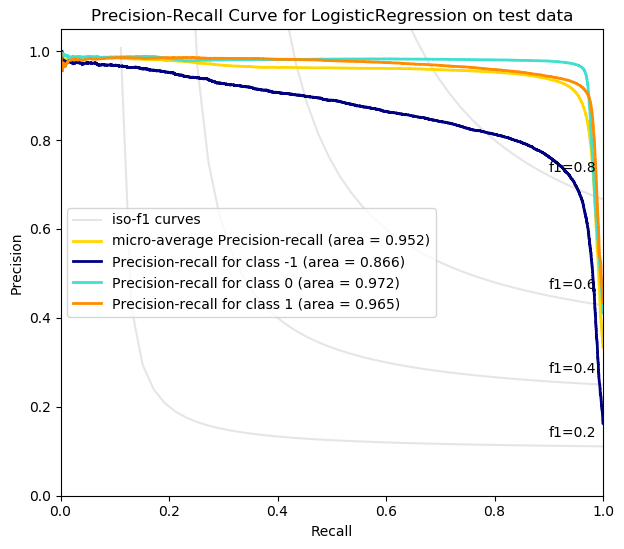
\includegraphics[width=0.95\columnwidth]{figures/PrecisionRecall_LogisticRegression_test.png}} & 
\subfloat[Precision vs. Recall for Linear SVC \label{fig:pr-svc}]{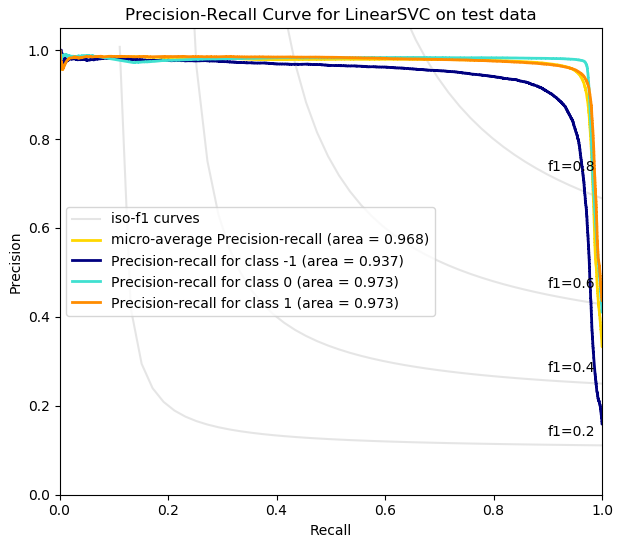
\includegraphics[width=0.95\columnwidth]{figures/PrecisionRecall_LinearSVC_test.png}}
\end{tabular}
\end{figure*}
In order to measure the performance of different classification techniques on the YouTube data, we split the data from US comments into train and dev subsets. To generate the train set, we randomly choose $80\%$ of the comments from each of the three categories. The remaining comments form the dev set. We use $20\%$ of the GB comments as the test set. 
To compare the performance of different methods we use accuracy, precision, recall and $F1$ score. 
Accuracy is defined as:
\begin{equation*}
\mathrm{Accuracy} = \frac{\left|\mathrm{True\:predictions}\right|}{\left|\mathrm{All\:predictions}\right|}.
\end{equation*}
Precision indicates what fraction of the predictions made by a classifier are true.
\begin{equation*}
P = \frac{\left|\mathrm{True\:positives}\right|}{\left|\mathrm{Predicted\:positives}\right|}.
\end{equation*}
Recall indicates what fraction of the population of a class are classified correctly by a classifier.
\begin{equation*}
R = \frac{\left|\mathrm{True\:positives}\right|}{\left|\mathrm{Real\:positives}\right|}.
\end{equation*}
Precision-recall is often used to determine the success rate of a model when the classes have imbalanced population .  
Once the precision and recall metrics are obtained, we compute the harmonic mean also known as F1 score. F1 score is defined as:
\begin{equation*}
F1 = \frac{2PR}{P + R},
\end{equation*}
where P is the precision and R is the recall. The maximum value of $F1$ score is $1$ which means the model reached perfect precision and recall.

In case of multi-class classification problems, we first need to binarize the output. 
We take a one-vs-all approach to deal with this issue. Precision and recall can then be generalized to the case of multi-class classification using a technique called micro-averaging. In this technique, every quantity in the above equations is replaced with the sum of corresponding quantities in all classes. For example, $\left|\mathrm{True\:positives}\right|$ is converted to $\left|\mathrm{True\:positives}_{\mathrm{class1}}\right| + \left|\mathrm{True\:positives}_{\mathrm{class2}}\right|$.

Table~\ref{tab:accuracy} shows the accuracy measured on train and test sets. Naive Bayes classifier has the worst performance among all methods. This result was predictable as the conditional independence condition required by the Naive Bayes classifier is not satisfied in this dataset. In particular, the conditional probabilities of two words happening in a comment given the category of the comment are not independent from one another. On this dataset, SVM classifier has the best performance. It is observed that the other three models have reasonable accuracy while LinearSVC outperforms the others. 

Figure~\ref{fig:pr-lr} shows the Precision-Recall curve of Logistic Regression while Figure~\ref{fig:pr-svc} shows that of LinearSVC. It is seen that precision and recall have an inverse relationship with each other. It happens because the more positive cases an algorithm reports, the more it is likely to report all positives points of the dataset (high recall), but it can also report more false positives (lower precision) and vice versa. Also, as the area under the curve increases, the precision and recall increase, where the increase of precision represents the increase of true positive rate and increase of recall represents the decrease of false negative rate. 
 
We optimized the regularization term of all models using cross validation. For sentiment analysis, the default values of Scikit performed well. These values can be found in the first column of Table~\ref{tab:params}. Note that regularization is proportional to $\alpha$ for Ridge regression and \textit{inverse} of $C$ for Softmax regression and Linear SVC.

\begin{figure}[tbh]%
\centering
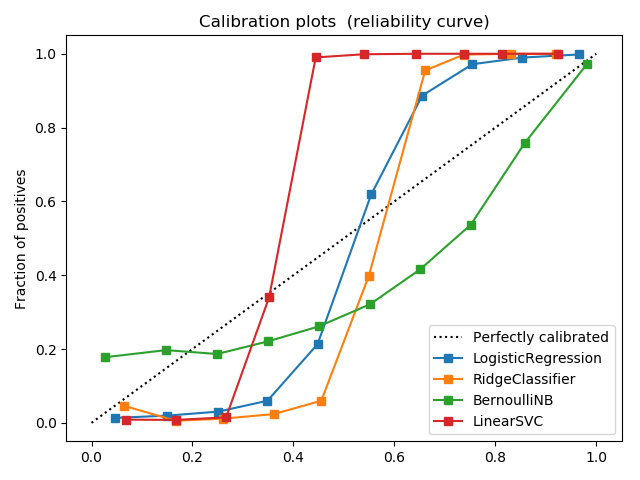
\includegraphics[width=0.9\columnwidth]{figures/calibration.png}%
\caption{Calibration curves}%
\label{fig:calibration}%
\end{figure}

\begin{figure}[tbh]%
\centering
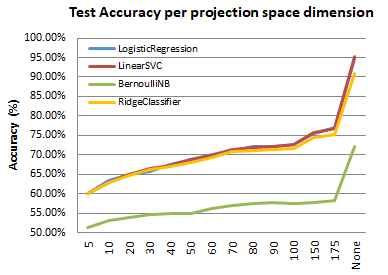
\includegraphics[width=0.9\columnwidth]{figures/dim_reduction_accuracy.png}%
\caption{Accuracy vs. project space dimensions}%
\label{fig:dim-reduction}%
\end{figure}
Figure~\ref{fig:calibration} shows the calibration curve of the aforementioned techniques. It is observed that Naive Bayes classifier is not well-calibrated over the range $[0,1]$. From among the remaining three methods, Logistic Regression is well-calibrated over the range $[0,1]$ and is in general better calibrated than the other two methods.


\subsection{Effect of Dimensionality Reduction}
\label{sec:dim-reduction}
In this set of experiments, we examined how dimensionality reduction can affect the accuracy of predictions. Dimension reduction is usually applied to reduce the complexity of computations. We apply TruncatedSVD to project TF-IDF features to fewer dimensions than those of the original TF-IDF feature space. We use TruncatedSVD rather than Principal Component Analysis (PCA) because the TF-IDF features are stored in a sparse matrix by the Scikit library which PCA cannot process. TruncatedSVD is very similar to PCA. However, the data is not centered around its mean in the former.
Figure~\ref{fig:dim-reduction} shows the accuracy of sentiment analysis with TruncatedSVD applied to TF-IDF features versus number of dimensions of the projection space. It is observed that accuracy increases with the number of dimensions. Nevertheless, with $175$ dimensions, it is still far from the case where no dimensionality reduction is applied. It seems that in this dataset, $175$ dimensions is not enough to project the data without loosing much information. We could not experiment with higher dimensions due to memory limitations of our desktops.

\begin{table}%
\centering
\begin{tabular}{|l|l|l|}
\hline
 & sentiment & category \\
\hline
Softmax Regression & $C = 1.0$ & $C = 1.0$ \\
\hline
Linear SVC & $C = 1.0$ & $C = 0.05$ \\
\hline
Ridge Classifier & $\alpha = 1.0$ & $\alpha = 10$\\
\hline
\end{tabular}
\caption{Optimal regularization constant}
\label{tab:params}
\end{table}

\subsection{Category Classification}
\label{sec:cat-exp}
\begin{figure*}[tbh]%
\centering
\begin{tabular}{cc}
\subfloat[category classification accuracy using comments \label{tab:cat-comment}] {
\begin{tabular}{|l|c|c|}
\hline
Model & Train Accuracy & Test Accuracy \\
\hline
Logistic Regression & $0.6070$ & $0.5322$ \\
\hline
Bernoulli NB & $0.4554$ & $0.4161$ \\
\hline
Ridge Classifier & $0.6578$ & $0.5592$ \\
\hline
Linear SVC & $0.6895$ & $0.5780$ \\
\hline
\end{tabular}} &

\subfloat[category classification accuracy using tags\label{tab:cat-tag}] {
\begin{tabular}{|l|c|c|}
\hline
Model & Train Accuracy & Test Accuracy \\
\hline
Logistic Regression & $00.9987$ & $0.7139$ \\
\hline
Bernoulli NB & $0.4909$ & $0.3835$ \\
\hline
Ridge Classifier & $0.9955$ & $0.7286$ \\
\hline
Linear SVC & $0.9954$ & $0.7286$ \\
\hline
\end{tabular}}
\end{tabular}
\caption{Category prediction of YouTube videos}%
\label{fig:cat-prediction}%
\end{figure*}
In this section, we report the results of experiments for category classification using TF-IDF comment features. In the first experiment we try to detect the category of the video corresponding to a comment using the TF-IDF features of the comment.  We used the same train, dev and test datasets as those used for sentiment analysis. Table~\ref{tab:cat-comment} shows the accuracy of different techniques for category classification using comment features. It is seen that the results are not as good as sentiment classification. Of course, considering there are $15$ categories versus $3$ sentiment classes, this problem is deemed to be harder. Yet, the probability of a successful random category guess is only $1/15 \: (6.7\%)$. Consequently, category prediction based on TF-IDF features of comments is still a big improvement over random guessing.

We then conducted category classification based on video tags. To split the data into train, dev and test, we randomly chose $80\%$ of the videos and their associative tags as the train dataset. The remaining $20\%$ of videos were split equally into dev and test sets. We did not use GB videos in this experiment as their categories were not the same as those of US videos.
Table~\ref{tab:cat-tag} summarizes the results. It is observed that tags can predict the category with much higher accuracy. Note that tags are considered a property of videos while TF-IDF features are a property of comments. In addition, tags are explicitly chosen to classify the videos. As a result, it is expected that they be less noisy and more directly relevant to the content of the video leading to higher accuracy.
Although category prediction by tags has higher accuracy, each of these two methods can be used in different scenarios depending on the data at hand. If we have clean data about videos with tags at our disposal and the learning task is to classify the videos into multiple categories, then tags are the better option. However, if all we have is comments and the association between comments and videos is not available (ex. the database containing videos is lost) and the prediction task is to find what category of movies a comment is about, then we have to content with category classification using comment features. The optimal regularization constant for category classification based on tags is denoted in the second column of Table~\ref{tab:params}.

In another experiment, we examined the effect of the number of categories on accuracy. Intuitively, the larger the number of categories, the more difficult the classification problem is expected to be. To experiment this intuition, we created a list of categories with ascending order of each category population. We considered the first $2$ categories, that is, the two categories with greatest number of videos, ignored the remaining videos in train and test set and measured the accuracy. The same experiment was repeated for $3, 4, \ldots, 15$ categories.
Figure~\ref{fig:cat-num-test} shows how test accuracy decreases by increasing the number of categories.
\begin{figure}%
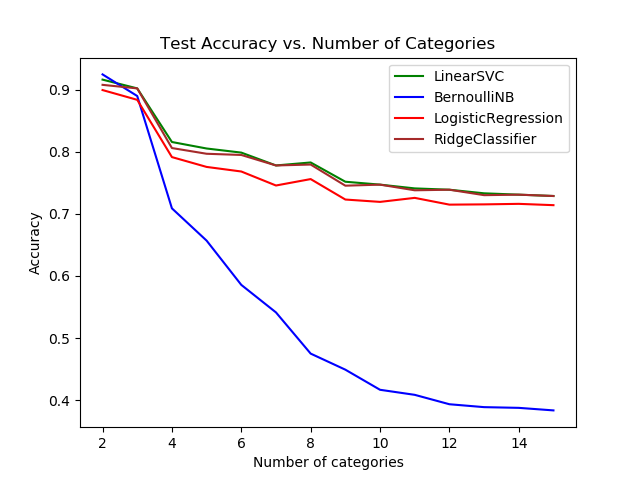
\includegraphics[width=1.0\columnwidth]{figures/cat-num-test-acc.png}%
\caption{Accuracy versus projection space dimensions}%
\label{fig:cat-num-test}%
\end{figure}